\documentclass{acm_proc_article-sp}

\usepackage{graphicx}
\usepackage{hyperref}

\usepackage{framed}

\newenvironment{cframed}[1][blue]
  {\def\FrameCommand{\fboxsep=\FrameSep\fcolorbox{#1}{white}}%
    \MakeFramed {\advance\hsize-\width \FrameRestore}}
  {\endMakeFramed}

\usepackage{xcolor}         % colors
\definecolor{scarlet}{HTML}{FF2400}

\begin{document}

\title{Roadmaps in Peer Learning for Sustainable Learning Design}

\numberofauthors{6} %  in this sample file, there are a *total*
% of EIGHT authors. SIX appear on the 'first-page' (for formatting
% reasons) and the remaining two appear in the \additionalauthors section.
%
\author{
% You can go ahead and credit any number of authors here,
% e.g. one 'row of three' or two rows (consisting of one row of three
% and a second row of one, two or three).
%
% The command \alignauthor (no curly braces needed) should
% precede each author name, affiliation/snail-mail address and
% e-mail address. Additionally, tag each line of
% affiliation/address with \affaddr, and tag the
% e-mail address with \email.
%
% 1st. author
\alignauthor
Joseph Corneli\\
\affaddr{Knowledge Media Institute}\\
\affaddr{The Open University}\\
\affaddr{Milton Keynes, UK}\\
\email{joseph.corneli@open.ac.uk}
% 2nd. author
\alignauthor
Charles Jeffrey Danoff\\
\affaddr{Mr Danoff's Teaching Laboratory}\\
\affaddr{Chicago, IL}\\
\email{charles@danoff.org}
% 3rd. author
\alignauthor
Fabrizio Terzi \\
\affaddr{Bergamo HUB}\\
\affaddr{Bergamo, IT}\\
\email{fabrizio.terzi@gmail.com}
\and  % use '\and' if you need 'another row' of author names
% 4th. author
\alignauthor Charlotte Pierce \\
\affaddr{Pierce Press} \\
\affaddr{Arlington, MA}\\
\email{charlotte.pierce@gmail.com}
% 5th. author
\alignauthor John Graves \\
\affaddr{Auckland University of Technology}\\
\affaddr{Auckland, NZ}\\
\email{jgraves@aut.ac.nz}
% 6th. author
\alignauthor R\'egis Barondeau \\
\affaddr{Universit\'e du Qu\'ebec \`a Montr\'eal}\\
\email{regis.barondeau@mac.com}
}

% There's nothing stopping you putting the seventh, eighth, etc.
% author on the opening page (as the 'third row') but we ask,
% for aesthetic reasons that you place these 'additional authors'
% in the \additional authors block, viz.
% \additionalauthors{Additional authors: John Smith (The Th{\o}rv{\"a}ld Group,
% email: {\texttt{jsmith@affiliation.org}}) and Julius P.~Kumquat
% (The Kumquat Consortium, email: {\texttt{jpkumquat@consortium.net}}).}
% \date{30 July 1999}

% Just remember to make sure that the TOTAL number of authors
% is the number that will appear on the first page PLUS the
% number that will appear in the \additionalauthors section.

\maketitle
\begin{abstract}

Following a year of productive learning and work culminating in the first edition of The Peeragogy Handbook we reflect here on lessons learned and patterns uncovered. In the second half of the paper we outline our goal: to transition from an innovative theoretical project to a sustainable, easily replicable peer project problem solving accelerator dynamically measuring assessment.

\end{abstract}

%
%
% New Section note for visual aid while editing
%
%

\section*{Categories and Subject Descriptors}
[{\bf Applied computing}]: {Education}, {Collaborative learning};
[{\bf Applied computing}]: {Document management and text processing}, {Document preparation}---\emph{Hypertext / hypermedia creation};
[{\bf Information systems}]: {Information systems applications}, {Collaborative and social computing systems and tools}---\emph{Wikis}

\terms{Human Factors}

\keywords{Peer learning, peer-to-peer, print on demand} % NOT required for Proceedings

\section{The Peeragogy Project}

The Peeragogy Project is a group of adult learners trying to uncover
the most effective ways to do collaborative learning.  We have been
working together in an open online community since January, 2012.  

Our methodology is based on examining and recording how we learn and
work together, and on existing examples and theories of peer learning.
We encourage participants to building and share experiments and case
studies (e.g. the classroom intervention ``5PH1NX'', the virtual
development collaboration hosted by the Free Technology Guild, the new
Bergamo HUB which is intended to be a civic center and maker space).
As such, the project serves as a research-based distributed project
incubator.

This paper describes the qualitative aspects of participation in this
project.  Our findings can be used by other projects with a
collaborative focus, and a ``humanities-friendly'' accompaniment to
previous writing about collaboration in open source software
(\cite{OpenAdvice}, \cite{crowstonXdefiningX2003}), with a learning
focus that is missing from other more general discussions of online
community \cite{bacon2012art}.

One of the key issues we address in this paper is multiplicity of
narratives.  Nearly every participant in the project has a different
view of what it's about, how it is useful for them, and how useful it
is for them.  The primary motivators reported by participants in the
Peeragogy project include:
\begin{itemize}
\item Acquisition of training or support in a topic or field;
\item Building relationships with interesting people;
\item Finding professional opportunities through other participants;
\item Creating or bolstering a personal network;
\item More organized and rational thinking through dialog and debate;
\item Feedback about their own performance and understanding of the
  topic.
\end{itemize}

Each of those motivators can affect the vitality of the peeragogical
process and the end result for the individual participant.  In
addition to our own reports from our experience, this paper draws on
survey data to brings in the voices and views of less-involved members
our Google+ community ($N=250$, $RR=17\%$).

\section{Acknowledgements}

The Peeragogy project was instigated by Howard Rheingold, adapting the
Corneli and Danoff \cite{paragogy} work on Paragogy to build a
less-academic, more practical, DIY tract built a group of contributors
that included, in addition to the current authors: Bryan Alexander,
Paul Allison, Doug Breitbart, Suz Burroughs, Jay Cross, Julian Elve,
Mar\'ia Fernanda, James Folkestad, Kathy Gill, Gigi Johnson, Anna
Keune, Roland Legrand, Christopher Neal, Ted Newcomb, Stephanie
Parker, David Preston, Paola Ricaurte, Stephanie Schipper, and Geoff
Walker.

\begin{figure}
\begin{center}
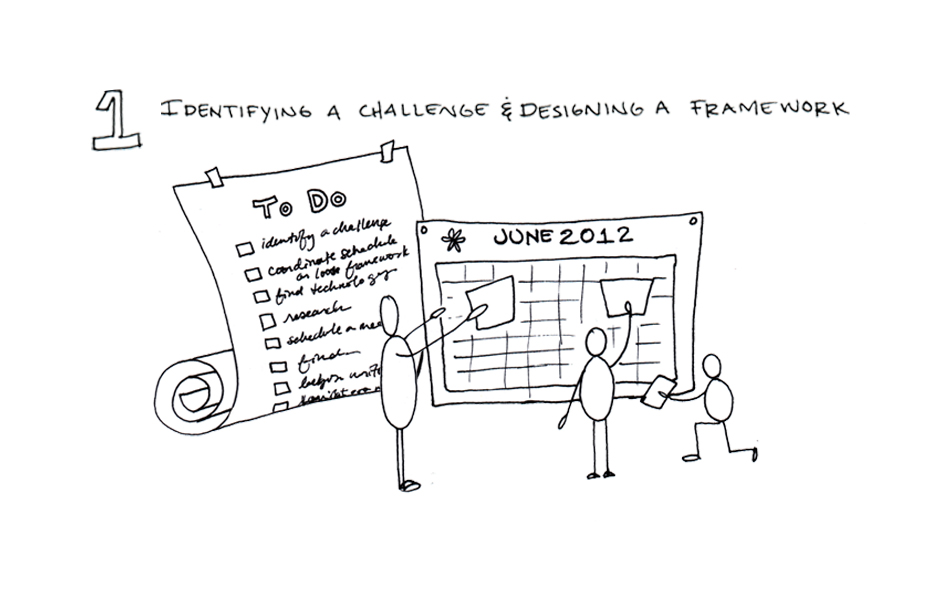
\includegraphics[width=.5\textwidth]{OpenBook1.jpg}
\vspace{-.7in}
\end{center}
\caption{Work by Amanda Lyons on ``Peeragogy in Action''
  \cite{PeeragogyinAction} \label{amanda}}
\end{figure}

\section{Problem Solved: The Peeragogy Handbook 1.0}

Peeragogy is a set of replicable techniques and patterns for effective
peer learning and problem solving.  Evidence that this can work comes
from our project: without the support of a unifying formal
institution, over the course of a year, a group of volunteers came
together and wrote a cohesive treatise on peer learning, far richer
than what any one of these people could have produced alone.

We utilized a variety of technologies to get the job done: live
meetings and a loose bureaucracy of teams and team leaders for
different sub-projects.  We elected to use the Creative Commons Zero
Public Domain Dedication for all of our work, to maximize the
potential for re-use.  Contributors submitted texts, images, and
videos, and in addition to our handbook, we prepared several external
presentations and publications (cf. Figure \ref{amanda}).

We used a blend of synchronous and asynchronous collaboration, and a
whole suite of tools: the Social Media Classroom, Diigo, Google Docs,
Google+, WordPress, LaTeX, Lulu, Twitter, Blackboard Collaborate, Git,
Google Hangouts, Mumble, and more.  

Each of these tools has its own pros and cons and fits a certain
purpose -- peeragogy is not bound to particular digital tools nor the
digital world at all.  For example, a physical interpretation was
given to the project by Anna, Paola, Gigi and Amanda who held a
workshop at the Open Knowledge Conference 2012 in Helsinki\footnote{
  \url{http://okfestival.org/peeragogy-handbook-workshop/} and
  \url{http://www.youtube.com/watch?v=P2UJrN58MVI}, leading to the
  peeragogy contribution to the Open Book \cite{PeeragogyinAction}.},
and again with the work-in-progress by Fabrizio to build a peer learning focused community center.\footnote{\url{http://paragogy.net/Bergamo_HUB:_il_potere_di_innovare_attraverso_la_collaborazione}}

Intuitively, there are bound to be difficulties for a group of peers studying a subject together, outside a traditional classroom or without a teacher. Indeed, peer learning is different from other forms of group effort, the proverbial ``barnraising'' for example, in which the persons involved can be presumed to know how to build barns - or at least to know someone who knows, and stand ready to take orders.  Typically, peers are not experts in learning, didactics, or in the subject they are studying, and are faced with multiple difficulties associated with putting together knowledge about the subject, assembling a suitable learning strategy, and communicating with one another \cite{paragogy}.  In addition to these \emph{a priori} barriers, we needed to create achievable common goals and overcome differences in timezone, different levels of English fluency, and varied levels of experience with technology, different writing styles, and different styles of engagement.

Our strategy was roughly to use each participant's difference as
points of strength.  In essence, we have high cognitive diversity,
and, since we all roughly agree about what we're aiming for in the
project and have allowed ourselves to be inspired by one another, far
less ``identity diversity'', in the sense that ``the more different we
are, the less we agree on what we would like to do''
\cite{Page2008difference}.  We've taken a similar ``open'' approach to
projects and tools, for instance, we've experimented with translation
on the MediaWiki powered Wikibooks platform, project organization with
the Federated Wiki and Trello.  The project has three main ``hubs'':
the Social Media Classroom, where we started writing, the Wordpress
site peeragogy.org, where we host the master copy of the handbook, and
our Google+ community.  Each new tool and contribution poses questions
about how to connect back to the overall flow of work and the book
outline.  It's hard to know in advance which experiments will work!

At a high level, the goal of producing a handbook explaining how other
peers could learn effectively with other peers on a given project kept
things cohesive, and gave us a standard of quality.  Producing the
book proved to be a viable method for researching and deepening our
understanding of peer learning.

Version 1.0 of the Peeragogy Handbook presents a range of techniques
that self-motivated learners can use to connect with each other and
develop stronger communities and collaborations.  We are continuing to
refine the book in the open, and we aim to publish Version 2.0 on
January 1, 2014.

In the mean time, we are also building on what we learned to
transition from an innovative theory-driven research project to a
sustainable and replicable peer produced problem solving accelerator.

\newpage
\subsection{What we learned 2012}

We've identified several basic and more elaborated patterns (in the
sense of \cite{Origins}, \cite{Tales}, \cite{vlissides1995design})
that describe ``the peeragogy effect''.

The central pattern is that of a Roadmap, which can apply at the
individual level, as a personal learning plan, or at a project
level.\footnote{See ``What are Learning Analytics?'' by George Siemens
  \url{http://www.elearnspace.org/blog/2010/08/25/what-are-learning-analytics/}
  for more on individual learner profiles as a context for developing
  and tracing progress on individual learning plans.}  The roadmap may
include a reason ``why'' \cite{sinek2009start}, exposition about the
goal, indicators of progress, a section for future work, and so forth.
Our initial roadmap for the project was the preliminaly outline of the
handbook; as the handbook approached publishability, we spun off
additional goals into a new roadmap for developing further aspects of
the
project.\footnote{\url{http://peeragogy.org/peeragogy-org-roadmap/}}

Group culture around maintaining and updating the roadmap define
project governance.  Other patterns flesh out the project's emergent
properties in a sort of ``agora'' of possibilities.

\hspace{.2in}
\begin{minipage}{.4\textwidth}
\begin{description}
\item[Roadmap] Plans for future work, direction towards a goal, dynamic
\item[Convene] \quad \\[-.1in]
\begin{itemize}
\item[\emph{Project}] Most projects involve learning!
\item[\emph{Guide}] Overviews expose the lay of the land collecting content
  and stories.
\end{itemize}
\end{description}
\end{minipage}

\hspace{.2in}
\begin{minipage}{.4\textwidth}
\begin{description}
\item[Organize] \quad \\[-.1in]
\begin{itemize}
\item[\emph{Roles}] Specialize and mix it up. Play to participants strengths
  and skills.
\item[\emph{Newcomer}] Create a guide for ``beginner's mind'' and help avoid
  need to bring new members up to speed each ``meeting.''
\item[\emph{Wrapper}] Consolidate and contain. Front end appearance to
  participants.
\end{itemize}
\end{description}
\end{minipage}

\hspace{.2in}
\begin{minipage}{.4\textwidth}
\begin{description}
\item[Cooperate] \quad \\[-.1in]
\begin{itemize}
\item[\emph{Heartbeat}] The ``heartbeat'' of the group keeps energy flowing.
\item[\emph{Capacity}] Know your limits, find ways to get other people
  involved.
\item[\emph{Moderation}] When leaders step back, dynamics can improve;
  moderator serves as champion and editor.
\item[\emph{Poll}] Invite brainstorming, collecting ideas, questions, and
  solutions.
\item[\emph{Patience}] Do not hold grudges and do not make pithy comments
  about team members or other institutions.
\item[\emph{Sacrifice}] Participants must be willing to sacrficice credit.
\end{itemize}
\end{description}
\end{minipage}

\hspace{.2in}
\begin{minipage}{.4\textwidth}
\begin{description}
\item[Assess]  \quad \\[-.1in]
\begin{itemize}
\item[\emph{Reuse}] Repurposing, tinkering, or creating from scratch?
\item[\emph{Discern}] Found a pattern? Give it a title and example.
\item[\emph{Believe}] Participants need to buy in to the idea or philisophy
  behind a project.
\end{itemize}
\end{description}
\end{minipage}

These patterns provide a natural framework for participatory design
and research in peer learning projects.  For example, can use them to
provide a terse profile for our project:

\begin{figure}[h]
\begin{cframed}[black]
{\bf Roadmap}: We aim to build a generally Wikipedia-like project for
learning.  We different from Wikiversity and P2PU because we're not
focusing on courses or learning materials, but on real-time support
for individual projects.  In this sense we are more like the
historical university. \\

\emph{Guide}: The Handbook is our guide for ourselves and newcomers. \\

\emph{Wrapper}: Christopher Tillman Neal has provided Weekly or
Bi-Weekly summaries throughout the duration of the project. \\

\emph{Heartbeat}: Charlotte Piece has hosted regular collaborative
editing sessions using Google Hangouts and Google Docs. \\

\emph{Capacity}: The Social Media Forum is accessible only to logged in
users.  We've also made routine efforts to ``prune'' the list of
contributors by asking people to actively renew interest or leave.
This gives us a core group of active contributors. \\

\emph{Poll}: Google+ has been a place to bring in new ideas and weak
links to other projects. \\

\emph{Reuse}: We have not had to build any special-purpose software to
run the project.  \\

\emph{Believe}: Often, people who \emph{like} the project are not the
strongest contributors, but it is rewarding to have enthusiastic
readers.  We've worked hard to make it easy for people to ``convert''
into contributors; there is qualitatively a missionizing aspect to the
project, and we have drawn on previous work in this space to refine
our approach \cite{Bridges}. 
\end{cframed}
\vspace{-.2in}
\caption{Terse description of the Peeragogy project using our pattern catalog}
\end{figure}

\subsection{Peer Survey}

In an effort to document ``the paths in the grass'' \cite{Wall} that come from unexpected links between different things in our successful publication of last year's Handbook we prepared a short survey for Peeragogy project participants. We asked people how they had participated (e.g Signing up for access to the Social Media Classroom and mailing list, Joining the Google+ Community, Authoring articles, etc.), and what goals or interests motivated their participation. We asked them to describe the Peeragogy project itself in terms of its aims and to evaluate its progress over the first year of its existence. As another measure of ``investment'' in the project, we asked, with no strings attached, whether the respondent would consider donating to the Peeragogy project. This survey was circulated to 223 members of the Peeragogy Google+ community, both en masse, and with individual +{\sl Name} call-outs, as well as to the currently active members of the Peeragogy mailing list.

The outline of the project's purpose ranged from the general: ``How to
make sense of learning in our complex times'' -- to much more
specific:

\begin{quote}
Push education further, providing a toolbox and [techniques] to
self-learners. In the peeragogy.org introduction page we assume that
self-learners are self-motivated, that may be right but the Handbook
can also help them to stay motivated, to motivated others and to face
obstacles that may erode motivation.
\end{quote}

Considering motivation as a key factor, it is interesting to observe
how various understandings of the project's aims and its flaws
intersected with personal motivations. For example, one respondent
(who had only participated by joining the Google+ community) was:
``[Seeking] [i]nformation on how to create and engage communities of
interest with a shared aim of learning.''

More active participants justified their participation in terms of what they get out of taking an active role, for instance:

\begin{quote}
Contributing to the project allows me to co-learn, share and co-write ideas with a colourful mix of great minds. Those ideas can be related to many fields, from communication, to technology, to psychology, to sociology, and more.
\end{quote}

The most active participants justified their participation in terms of
beliefs or a sense of mission:

\begin{quote}
Currently we are witnessing many efforts to incorporate technology as
an important tool for the learning process. However, most of the
initiatives are reduced to the technical aspect (apps, tools, social
networks) without any theoretical or epistemological
framework. Peeragogy is rooted in many theories of cooperation and
leads to a deeper level of understanding about the role of technology
in the learning process. I am convinced of the social nature of
learning, so I participate in the project to learn and find new
strategies to learn better with my students.
\end{quote}

Or again:

\begin{quote}
I wanted to understand how ``peer production'' really works. Could we
create a well-articulated system that helps people interested in peer
production get their own goals accomplished, and that itself grows and
learns? Peer production seems linked to learning and sharing - so I
wanted to understand how that works.
\end{quote}

They also expressed criticism of the project, implying that they may feel rather powerless to make the changes that would correct course:

\begin{quote}
Sometimes I wonder whether the project is not too much `by education specialists for education specialists'. I have the feeling peer learning is happening anyway, and that teens are often amazingly good at it. Do they need `learning experts' or `books by learning experts' at all? Maybe they are the experts. Or at least, quite a few of them are.
\end{quote}

Another respondent was more blunt:

\begin{quote}
What problems do you feel we are aiming to solve in the Peeragogy
project? We seem to not be sure. How much progress did we make in the
first year? Some..got stuck in theory.
\end{quote}

But, again, it's not entirely clear how the project provides clear pathways for contributors to turn their frustrations into changed behavior or results. Additionally we need to be entirely clear that we are indeed paving new ground with our work. If there are proven peer learning methods out there we have not examined and included in our efforts, we need to find and address them. Peeragogy is not about reinventing the wheel.

It's also not entirely clear whether excited newbies will find pathways to turn their excitement into shared products or process. For example, one respondent (who had only joined the Google+ community) had not yet introduced their fascinating projects publicly:

\begin{quote}
I joined the Google+ community because I am interested in developing peer to peer environments for my students to learn in. We are moving towards a community-based, place-based program where we partner with community orgs like our history museum for microhistory work, our local watershed community and farmer's markets for local environmental and food issues, etc. I would love for those local efforts working with adult mentors to combine with a peer network of other HS students in some kind of cMOOC or social media network.
\end{quote}

Responses such as this highlights our need to make ourselves available to hear about exciting new projects from interested peers, simultaneously giving them easier avenues to share. Our work on developing a peeragogy accelerator in the next section is an attemt to address this situation.

\subsection{Survey Analysis}

Clearly, many participants will have intermediate levels of investment -- basically ``social consumers'' of the project as a ``product''. However, if we think about the metaphor of a college or university, this description also applies to most members of the student body, who are physically present only for a brief portion of the institution's history, and who may not join the student government etc. A blueprint for a distributed university or peers we will discuss briefly in the conclusion perhaps named ``Peeragogy.EDU''\footnote{See \url{http://peeragogy.org/knight-foundation-prototype-fund-proposal-unfunded/}} should include plenty of room for people who take a less involved role. Nevertheless, integrating some of these light-weight contributions (like blog posts about the ideas) would be an important role for more active participants to take on.

Some of the big challenges can be parsed out using our high-level patterns. First, in our work, we uncovered pretty much everyone needs a team. Building off that, these issues could define new project ``roadmaps'' and ``teams'':

\begin{description}
\item[Cooperate] ~ How to build a really strong collaboration?

A team is not a group of people who work together. A team is a group of people who trust each other...

\item[Convene] ~ How to build a more practical focus?

The insight that the project will thrive if people are working hard on their individual problems and sharing feedback on the process seems like the key thing going forward. This feels valuable and important.

\item[Organize] ~ How to connect with motivated newcomers?

I just came on board a month ago. [...] I am designing a self organizing learning environment (SOLE) or PLE/PLN that I hope will help enable communities of life long learners to practice digital literacies.

\item[Assess] ~ How to be effective and relevant?

I am game to also explore ways to attach it to spaces where funding can flow based on real need in communities.
\end{description}

The basic workflow in the project -- discussing ideas, condensing them into written handbook sections, annotating them with new resources in informal discussion, reevaluating and rewriting -- seems relatively sustainable, as long as we have community members and editors who are willing to do the work. However, the long-term relevance of the project will come from building workflows that are less self-referential and more applied. With the current foundation in theory and examples from literature and day-to-day activities of participants, we are prepared to be a more effective peer-produced accelerator for peer learning and peer production projects. The kinds of critical questions elaborated above would tend to apply to other projects as well.

\begin{cframed}[scarlet]
\subsection{Looking backward}

We can also draw on the answers to our initial round of questions (a
``pilot study'')\footnote{\url{http://peeragogy.org/organize/}} [TODO
  if someone has time - quick copy and paste]
\end{cframed}

\section{The Peeragogy Accelerator}

Having piloted the peeragogy patterns as a research method for
understanding the peeragogy project itself, work is now underway to
apply them in another peer learning and peer production community,
PlanetMath, in the context of evaluating socio-technical change
associated with a public beta of new software for the decade-old site.

I would emphasize the transition from ``innovative project'' in
``sustainable learning design'' in short, we've been doing ``peer
support'' and ``critical thinking'' all along:

\begin{paragraph}{Example}
Joe and Charlie made a simple peer support pact outside of P2PU to sit
in on each others courses $\rightarrow$ discussions $\rightarrow$
papers $\rightarrow$ some of the seeds for the Peeragogy project.
\end{paragraph}

What makes Peeragogy different:
\begin{itemize}
\item we're not just offering content
\item we're also not offering ``classes'' (or a place to organize classes)
\item we're working at a higher level, more strategic
\item we're focusing on people instead of topics/subjects; if we have
  a common topic it is something like ``leadership led team skills''
\end{itemize}

\subsection{Pilot: ``PeerPub-U''}

Drawing on the experience and skills of its 108+ members, Independent
Publishers of New England's (IPNE) plans to build an open learning and
support network (a.k.a. PeerPubU, or ``Peer Publishing University'')
to address issues in independent publishing and provide education to
its members - part of its stated mission. IPNE facilitators hope that
this network will dovetail with other planned membership-building
efforts and help raise the standards and maximize success of indie
publishers in New England in this fast-changing business sector.

On Jan. 26, 2013, regional independent publishers and authors attended
the IPNE.org greater Boston branch meeting in Arlington, MA, billed as
a ``plenary session'' for PeerPubU. In addition to the live in-person
meeting, Peeragogy Handbook team members Gigi Johnson (Los Angeles,
US), Roland Legrand (Antwerp, Belgium) and Anna Keune (Helsinki,
Finland) joined via Google+ Hangout.  Plenary meeting observations:

At the meeting, IPNE President Tordis Isselhardt suggested a
Peeragogy-style effort might more likely meet with success if the
organization's members rallied around a specific project, perhaps an
``Independent Publishing Handbook,'' (like the Peeragogy Handbook) in
addition to creating resource repositories and sharing of expertise as
individuals' challenges arise.

Brainstorming ways to sustain motivation, members suggested that the
108 members of the association could earn authorship credit for
contributing articles and editor credit for working on the manuscript;
and could spin off their own chapters as stand-alone, profit-making
publications.  Members agreed to set up the project in IPNE's Basecamp
content-management platform. Members who express interest at the
branch meetings are regularly added. The Basecamp tally was 12
self-selected participants by March, 2013.

Peeragogues attending noted that there are facilitators, but not an
overall leader, of peer-learning efforts, and suggested that potential
contributors and facilitators prepare by visiting peeragogy.org and
extracting practices and patterns that might work best for IPNE.

IPNE officers at the meeting perked up at the suggestion that
``PeerPubU'' might become a case study in future editions of the
Peeragogy Handbook.

Live, in-person development sessions of the pilot Peeragogy project
take place at IPNE Greater Boston Regional Branch meetings on a
monthly basis, and an online video meeting platform is in development.

\subsection{PlanetMath}

Team member Joe Corneli ...

\subsection{The Uncertainty Principle}

Team member Charlie Danoff...

\subsection{Bergamo}

Team member Fabrizio Terzi is seeking to put Peeragogy in Action via a
HUB-inspired\footnote{\url{http://www.the-hub.net/}} Laboratory
Project Art \& Open Technology Incubator.  He is drawing on
peeragogical patterns and his peer learning network to develop an
application to submit to the Bergamo, Italy Art \& Tourism Council.

\subsection{More possible ideas for this section}

Also, how will we use what we learned to make 2013 better? (use
Peeragogical discoveries to improve the Peeragogy Handbook, Project,
spin-off and partner projects, etc.)

As we move into year two and an updated Handbook, we focus on translations and formalizing peeragogical patterns for problem solving; i.e., how can we (and other peers) use our ideas to better solve problems facing us directly.

In the course of this paper we will examine peeragogical applications to an online Math web cornucopia, Chicago based zine and a New England Independent Publishers association. The main problem we in 2013 and here in this paper are trying to solve is seeing if peeragogical patterns of transparency, accountability and efficiency can help us individually with pressing project problems. Specifically we seek to transition from an innovative theoretical project to a sustainable, easily replicable (peer project) problem solving accelerator.

%
%
% New Section note for visual aid while editing
%
%




\section{Conclusion}

Could this be useful to programmers at WikiSym as a way for them to
crowdsource their documentation?

This paper can be thought of as a moment in time of the Peeragogy Project, sort of like a financial statement (e.g. Balance Sheet) we want to understand where the money/learning's been going over the past year to budget learning for next year

Future steps
Outreach

Individuals have a lot of motivation, which is great, but they may need some support even if they are ``self-starters''.

``If you want to go fast, go alone, if you want to go far go together.''
We tend to need clear outputs, some form of assessment (e.g. a paper,
a talk, a thesis, a ``masterpiece'')
Documenting the more distributed knowledge process
e.g. you can watch a talk online

\begin{center}
*
\end{center}

Going forward we need to record data better -> (discussion with
R\'egis about
this)\footnote{\url{https://plus.google.com/u/0/101437188321463196206/posts/eUxkDqEAmvG}}
-> can we move towards some sort of learning achieved by hour metric?

The main point, I think, is, this one: What are the methods we've
identified that will help us make progress towards our goals?

\paragraph{Hypothesis 1}
In a peeragogy environment the 90-9-1 principle doesn't make sense.

\paragraph{Hypothesis 2} The long tail rule applies - This may validate
an other point in the section ``managing participation''.

\paragraph{Hypothesis 3} Most contributors influence the structure of the site not only the content (meaning re-organize the links over time) - I my wiki experience I see often a bunch of architectes create the structure and users follow it.

\paragraph{Hypothesis 4} Peer learning projects need to find the right balance of freedom, interest and bureaucracy.

I had an interesting idea about the power law of participation. The 90/10/1 breaks down when you work with small groups (like 1 person) -- and I'm guessing that the ``long tail'' is much longer (and skinnier) in G+ than in SMC. However, it's not necessarily that fat in SMC either.

Also, again, ``quality'' seems at least as important as ``quantity''... 

A ``phenomenological approach'': what is it like to participate or to have participated in the project?


We can start filling in ideas about these points asynchronously, as Charlie has started below. (Thanks Charlie!)

\subsection{Paragogical Action Review}

This aspect of the paper would hearkens back to the paragogy paper
that Joe and Charlie presented at OKCon 2011, further refined with our
experience at e/merge 2012.  Thinking longitudinally, we can ask: have
we learned anything since ``our P2PU days''?

\paragraph{Review what was supposed to happen}

\paragraph{What happened / is happening?}

\paragraph{What is right or wrong with what we're doing / have done?}

\paragraph{What did we learn or change?}

\paragraph{How can we learn this experience to improve next time?}

Charlie: can we move to using a higher percent of Free Software tools?
(more likely our work can be shared, remixed \& properly stored?).

%
% The following two commands are all you need in the
% initial runs of your .tex file to
% produce the bibliography for the citations in your paper.
% (Uncomment to reproduce the .bbl file if needed!)

% \bibliographystyle{abbrv}
% \bibliography{bib}  % sigproc.bib is the name of the Bibliography in this case

\begin{thebibliography}{10}

\bibitem{Origins}
C.~Alexander.
\newblock The origins of pattern theory, the future of the theory, and the
  generation of a living world,, 1996.

\bibitem{bacon2012art}
J.~Bacon.
\newblock {\em The art of community: Building the new age of participation}.
\newblock O'Reilly Media, 2012.

\bibitem{paragogy}
J.~Corneli and C.~J. Danoff.
\newblock Paragogy.
\newblock In S.~Hellmann, P.~Frischmuth, S.~Auer, and D.~Dietrich, editors,
  {\em Proceedings of the 6th Open Knowledge Conference}, Berlin, Germany,
  2011.

\bibitem{PeeragogyinAction}
J.~Corneli, A.~Keune, C.~J. Danoff, and A.~Lyons.
\newblock Peeragogy in action.
\newblock In {\em The Open Book}, pages 80--87. The Finnish Institute in
  London, 2013.

\bibitem{crowstonXdefiningX2003}
K.~Crowston, H.~Annabi, and J.~Howison.
\newblock Defining open source software project success.
\newblock In {\em Proceedings of the 24th international conference on
  information systems (icis 2003)}, pages 327--340. Citeseer, 2003.

\bibitem{Wall}
A.~Dougherty.
\newblock Gluing the web together: An interview with {L}arry {W}all.
\newblock {\em ZD Internet User}, 1998.

\bibitem{Tales}
R.~P. Gabriel.
\newblock {\em Patterns of Software}.
\newblock Oxford University Press, New York, 1996.

\bibitem{Bridges}
D.~McGavran.
\newblock {\em The Bridges of God}.
\newblock World Dominion Press, 1955.

\bibitem{Page2008difference}
S.~Page.
\newblock {\em The Difference: How the Power of Diversity Creates Better
  Groups, Firms, Schools, and Societies (New Edition)}.
\newblock Princeton University Press, 2008.

\bibitem{OpenAdvice}
L.~Pintscher, editor.
\newblock {\em Open Advice}.
\newblock lulu.com, 2012.

\bibitem{sinek2009start}
S.~Sinek.
\newblock {\em Start with why: How great leaders inspire everyone to take
  action}.
\newblock Portfolio, 2009.

\bibitem{vlissides1995design}
J.~Vlissides, R.~Helm, R.~Johnson, and E.~Gamma.
\newblock Design patterns: Elements of reusable object-oriented software.
\newblock {\em Reading: Addison-Wesley}, 49, 1995.

\end{thebibliography}


\balancecolumns


\end{document}
